\newpage
\section{Auswertung}
\label{sec:Auswertung}
\subsection{Bestimmung von Leerlaufspannung und Innenwiderstand}
In Tabelle \ref{tab:MZ} sind Klemmenspannung $U_\mathup{k}$ und Belastungstrom $I$ der Monozelle bei Gleich- und Gegenspannung, gemessen bei variablem Belastungswiderstand $R_\mathup{a}$, aufgetragen. Tabelle \ref{tab:Recht_Sin} enthält die Daten der Messung mit Rechteck- und Sinusspannungsquelle.

\begin{table}
	\centering
	\sisetup{table-format=2.3}
	\begin{tabular}{S[table-format=1.3] S[table-format=1.2] S[table-format=1.3] S[table-format=1.2] }
	\toprule
	\multicolumn{2}{c}{Monozelle} &\multicolumn{2}{c}{Monozelle mit Gegenspannung} \\
	{$I/\:\si{\ampere}$} & {$U_\mathup{k}/\:\si{\volt}$} &{$I/\:\si{\ampere}$} & {$U_\mathup{k}/\:\si{\volt}$}\\
	\midrule
 0.050 & 1.20 & 0.030 & 1.80\\
 0.060 & 1.15 & 0.040 & 1.90\\
 0.070 & 1.10 & 0.090 & 2.10\\
 0.080 & 1.05 & 0.110 & 2.20\\
 0.090 & 1.00 & 0.120 & 2.30\\
 0.110 & 0.90 & 0.150 & 2.50\\
 0.130 & 0.80 & 0.180 & 2.60\\
 0.150 & 0.70 & 0.230 & 2.90\\
 0.200 & 0.40 & 0.270 & 3.10\\
 0.260 & 0.10 & 0.310 & 3.30\\
\\
	\bottomrule
	\end{tabular}
	\caption{Messdaten der Monozelle und der Monozelle mit Gegenspannung.}
	\label{tab:MZ}
\end{table}


\begin{table}
	\centering
	\sisetup{table-format=2.3}
	\begin{tabular}{S[table-format=1.1] S[table-format=0.3] S[table-format=1.3] S[table-format=1.2] }
	\toprule
	\multicolumn{2}{c}{Rechteckspannung} &\multicolumn{2}{c}{Sinusspannung} \\
	{$I_\mathup{eff}/\:\si{\milli{\ampere}}$} & {$U_\mathup{k}/\:\si\volt$} &{$I\mathup{eff}/\:\si{\milli{\ampere}}$} & {$U_\mathup{k}/\:\si{\volt}$}\\
	\midrule
 1.0 & 260 & 0.72 & 0.20\\
 1.1 & 255 & 0.38 & 0.25\\
 1.2 & 245 & 0.36 & 0.27\\
 1.4 & 235 & 0.32 & 0.30\\
 1.6 & 230 & 0.27 & 0.33\\
 1.9 & 215 & 0.22 & 0.35\\
 2.2 & 190 & 0.14 & 0.40\\
 2.7 & 160 & 0.11 & 0.42\\
 3.5 & 115 & 0.10 & 0.44\\
 4.1 &  80 & 0.09 & 0.45\\
\\
	\bottomrule
	\end{tabular}
	\caption{Messdaten mit Rechteck- und Sinusspannung vom RC-Generator .}
	\label{tab:Recht_Sin}
\end{table}


Werden die Messewerte der Spannung $U_\mathup{k}$ gegen die Stromstärke $I$ aufgetragen und eine lineare Ausgleichsrechnung ausgeführt,  können Innenwiderstand $R_\mathup{i}$ und Leerlaufspannung $U_0$ der verwendeten Spannungsquellen bestimmt werden.
Die verwendeten Volt- und Amperemeter besitzen eine in der weiteren Auswertung berücksichtigte  Unsicherheit von 3\%. Abbildung \ref{fig:MZ} zeigt Messwerte mit Fehlerbalken und Regressionsgeraden der Messung an der Monozelle mit Gleich- und Gegenspannung; Abbildung \ref{fig:Recht} und \ref{fig:Sin} stellen Messpunkte und Ausgleichsgeraden der Rechteck- und Sinusspannung dar.
\begin{figure}[h]
	\centering
	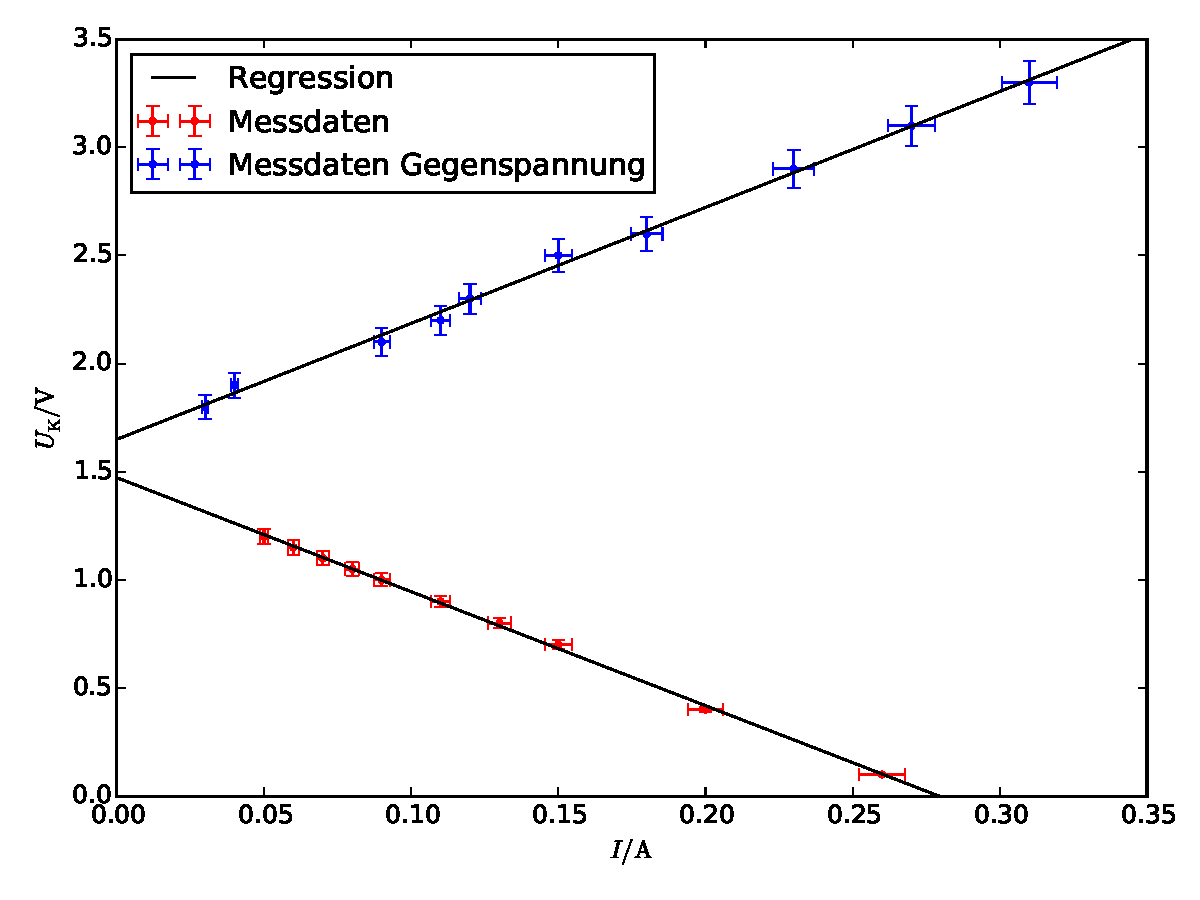
\includegraphics[width=\textwidth]{content/plot_MZ.pdf}
	\caption{Messwerte und Regression der Messung an der Monozelle mit und ohne Gegenspannung.}
\label{fig:MZ}
\end{figure}
\begin{figure}[h]
	\centering
	\label{fig:Recht}
	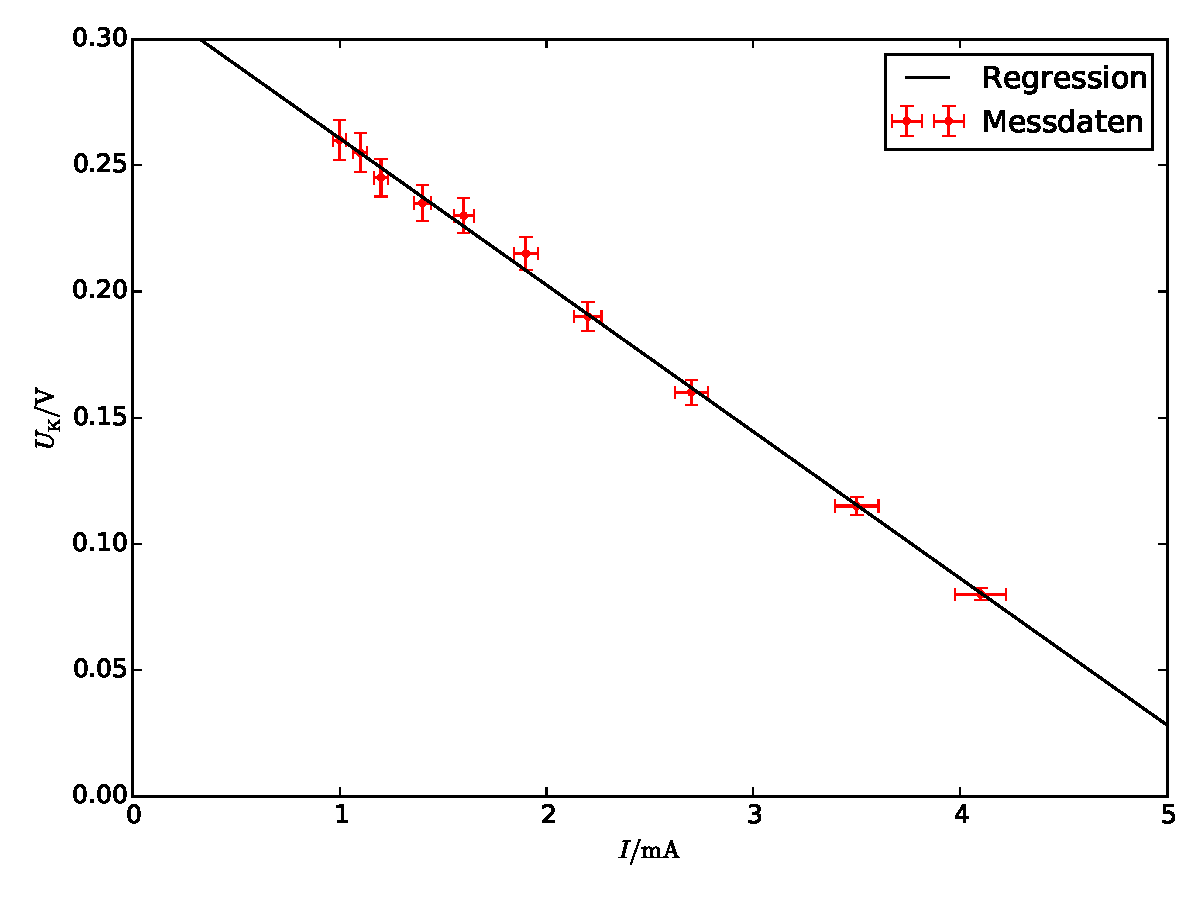
\includegraphics[width=\textwidth]{content/plot_Recht.pdf}
	\caption{Messwerte und Regression der Messung mit Rechteckspannungsqulle.}
\label{fig:Recht}
\end{figure}
\begin{figure}[h]
	\centering
	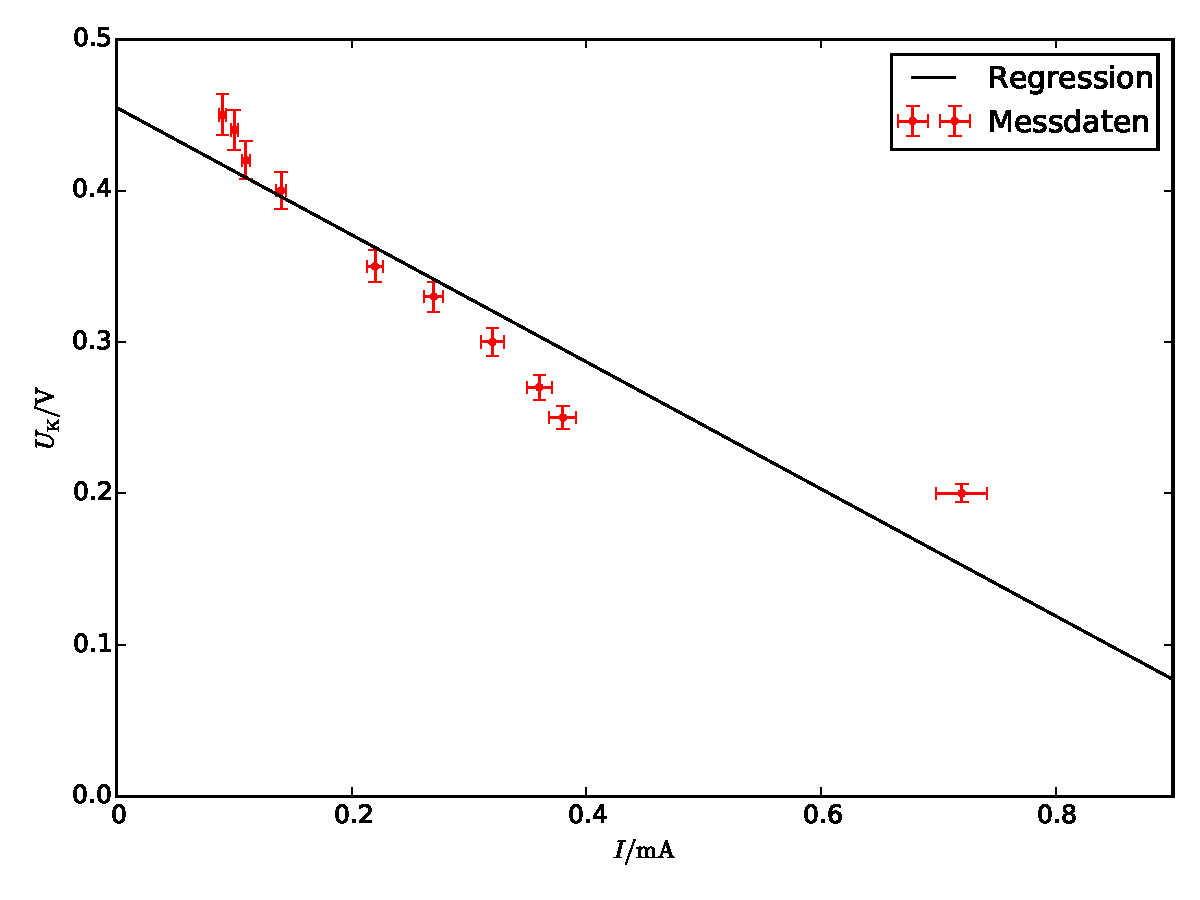
\includegraphics[width=\textwidth]{content/plot_Sin.pdf}
	\caption{Messwerte und Regression bei Messung mit Sinusspannungsquelle.}
	\label{fig:Sin}
\end{figure}

Es ergeben sich die Geradengleichungen mit berechneten Koeffizienten

\begin{align}
U_\mathup{k}=&(-5.27\pm0.06)\,\si{\ohm}\cdot I+(1.473\pm0.008)\,\si{\volt} &\text{Monozelle},\\
U_\mathup{k}=&(5.36\pm0.10)\,\si{\ohm}\cdot I+(1.650\pm0.018)\,\si{\volt} &\text{Gegenspannung},\\
U_\mathup{k}=&(-58\pm1)\,\si{\ohm}\cdot I+(0.3189\pm0.0024)\,\si{\volt} &\text{Rechteckspannung},\\
U_ \mathup{k}=&(-420\pm60)\,\si{\ohm}\cdot I +(0.455\pm0.018)\,\si{\volt} &\text{Sinusspannung}.
\end{align}
Daraus können nach Gleichung \eqref{eq:Klemmspannung} die in Tabelle \ref{tab:Ergebnisse} aufgetragenen Innenwiderstände und Leerlaufspannungen abgelesen werden. Dabei ist zu beachten, dass wegen der verwendeten Gegenspannung während der Messung an der Monozelle der Strom ein negatives Vorzeichen aufweist, da dieser in die entgegengesetzte Richtung fließt. Aufgrund der zweifachen Messung mit der Monozelle kann für diese das Mittel der Werte gebildet werden. 
\begin{table}
	\centering
	%\sisetup{table-format=3.3}
	\begin{tabular}{c c c}
	\toprule
	\multicolumn{1}{c}{Spannungsquelle} & \multicolumn{1}{c}{$R_\mathup{i}/\:\si{\ohm}$} & \multicolumn{1}{c}{$U_\mathup{0}/\:\si{\volt}$} \\
	\midrule
 \text{Monozelle} & 5.27\pm0.06 & 1.473\pm0.008\\
  \text{Gegenspannung} & 5.4\pm0.1 & 1.65\pm0.02\\
  \text{Mittelwert} &  5.32\pm0.08 & 1.56\pm0.01\\
  \text{Rechteckspannung} & 58\pm1 & 0.319\pm 0.003\\
  \text{Sinusspannung} & 420\pm60 & 0.46\pm0.02\\
	\bottomrule
	\end{tabular}
	\caption{Ergebnisse für Innenwiderstände und Leerlaufspannungen.}
	\label{tab:Ergebnisse}
\end{table}

\newpage
Die direkte Messung über das Voltmeter ergibt eine Leerlaufspannung \\$U_0=(1.5\pm0.05)\,\si{\volt}$, welche nur geringfügig vom Mittelwert in Tabelle \ref{tab:Ergebnisse} abweicht. Bei einem endlichen Eingangswiderstand $R_\mathup{V}=\SI{10}{\mega\ohm}$ des Voltmeters ergibt sich der systematische Fehler von $U_0=(8.2992\cdot10⁻⁷)\,\si{\volt}$ durch
\begin{equation}
\Delta{U_0}=\frac{R_\mathup{i}U_\mathup{k}}{R_\mathup{V}}.
\end{equation}

Bei dem Aufbau der Schaltung muss sorgsam darauf geachtet werden, dass das Voltmeter vor das Amperemeter geschaltet wird, damit tatsächlich die Spannung $U_\mathup{k}$ gemessen werden kann. Geschieht dies nicht, beeinflusst der Innenwiderstand des Amperemeters die Messung.
%%%%%%%%%%%%%%%%%%%%%%%%%%%%%%%%%%%%%%%%%%%%
%%%%%%%%%%%%%%%%%%%neue Subsection%%%%%%%%%%
%%%%%%%%%%%%%%%%%%%%%%%%%%%%%%%%%%%%%%%%%%%%
\newpage
\subsection{Leistung am Belastungswiderstand}

Es wird die am Belastungswiderstand $R_\mathup{a}=\frac{U_\mathup{k}}{I}$ umgesetzte Leistung $N$ der Monozelle ohne Gegenspannung betrachtet.
Werden die Größen gegeneinander aufgetragen, ergibt sich der in Abbildung \ref{fig:N} gezeigte Verlauf. Mit dem Innenwiderstand $R_\mathup{i}$ sowie der Leerlaufspannung $U_0$ aus Tabelle \ref{tab:Ergebnisse} kann nach Gleichung \eqref{eq:leistungsanpassung} eine Theoriekurve errechnet werden.

Mit den fehlerbehafteten Größen $U_\mathup{k}$ und $I$ ergeben sich mit der Gausschen Fehlerfortpflanzung die Fehler
\begin{equation}
\Delta{R_\mathup{a}}=\frac{U_\mathup{k}}{I}
\sqrt{\biggl(\frac{\Delta{U_\mathup{k}}}{U_\mathup{k}}\biggr)²+\biggl(\frac{\Delta{I}}{I}\biggr)²}
\end{equation}
und
\begin{equation}
\Delta{N}=U_\mathup{k}I\sqrt{\biggl(\frac{\Delta{U_\mathup{k}}}{U_\mathup{k}}\biggr)²+\biggl(\frac{\Delta{I}}{I}\biggr)²}.
\end{equation}
\begin{figure}[h]
	\centering
	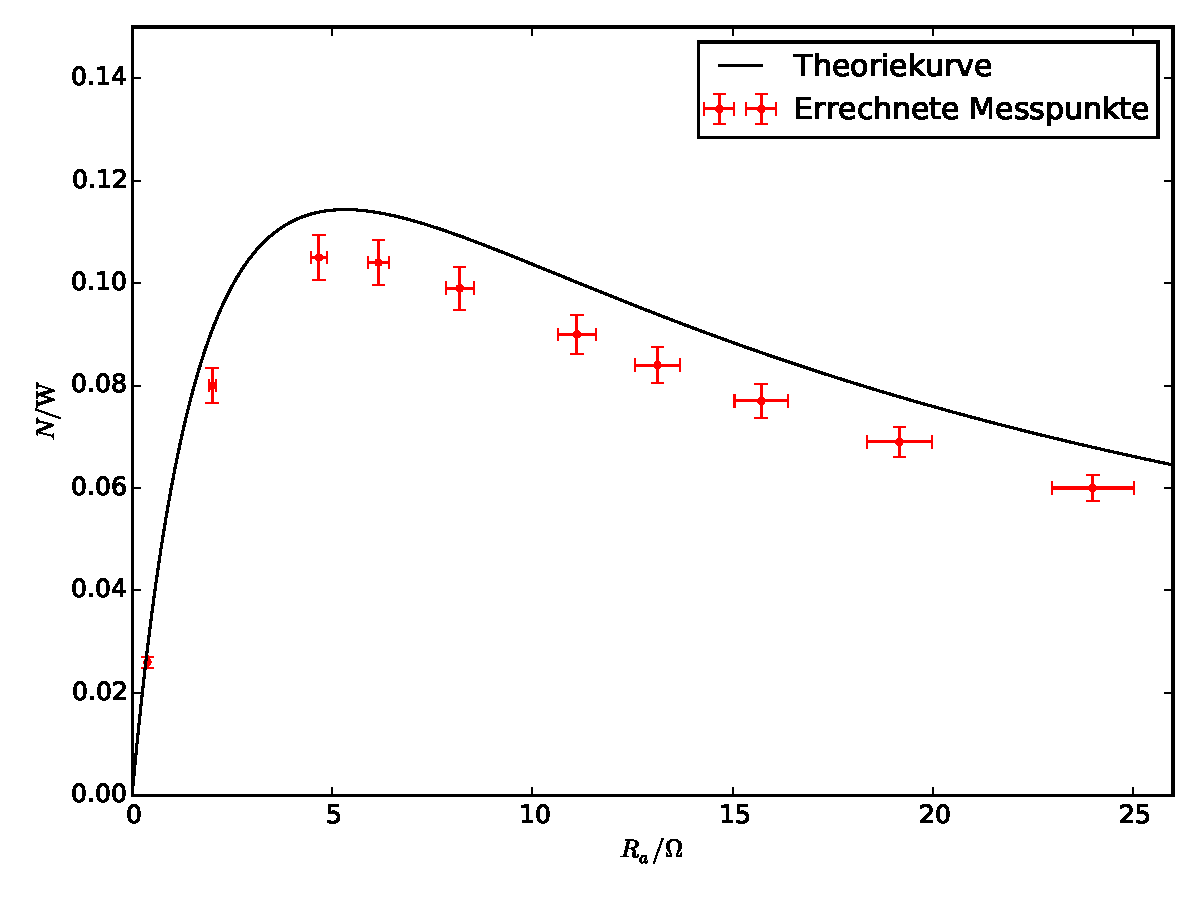
\includegraphics[width=\textwidth]{content/plot_L.pdf}
	\caption{Messwerte mit Fehlerbalken und Theoriekurve der am Belastungswiderstand abfallenden Leistung.}
\label{fig:N}
\end{figure}

Alle Messpunkte liegen trotz abgebildeter Standardabweichung in ungefähr gleicher Entfernung unter der Theoriekurve. Daraus kann auf einen systematischen Fehler geschlossen werden.
